\section{Project description}
\label{chapter1}

\subsection{Problem description}

The idea of our project is to build an automatic room ventilation. This could be used in a classroom or an office, for example. When the CO2 level in a room reaches a certain level, a window should automatically open and a fresh air fan should be switch on. After a certain lower CO2 level is reached and a certain run-on time has elapsed, the window should be closed and the fan switched off again.\\

The system is divided into 2 larger areas, one of which is a Raspberry Pi and the other is an Arduino. These two components are supposed to communicate with each other and exchange data via a secure Bluetooth connection. 

\subsection{Arduino}

The project part of the Arduino consists of the following hardware:

\begin{enumerate}[label*=\arabic*.]
    \item \label{hw.1} Arduino Nano 33 IoT 
    \item \label{hw.2} MiCS-VZ-89TE CO2 Sensor
    \item \label{hw.3} cabling
\end{enumerate}

The main task of the Arduino is data acquisition and data processing. It should measure the data via the co2 sensor, check its validity and then interpret it. Based on the values, their history and certain thresholds, the Arduino sends its current status to the Raspberry Pi every 10 seconds. This can be IDLE, OPEN or CLOSE. The status OPEN and CLOSE are sent once when the window is to be opened/closed and the fan is to be switched on/off.

\subsection{Raspberry Pi}

The project part of the Raspberry Pi consists of the following hardware:

\begin{enumerate}[label*=\arabic*.]
    \item \label{io.1} Raspberry Pi 4 Model B 8GB
    \item \label{io.2} 2x Mini Stepper Motor Kit ULN2003A with 28BYJ-48
    \item \label{io.3} potentiometer
    \item \label{io.4} cabling
\end{enumerate}

On the other hand, the Raspberry Pi is mainly responsible for device control. It receives the status of the Arduino every 10 seconds and works based on it. When the status is OPEN or CLOSE, it controls the motor for the window and the motor for the fan and turns them on/off. The potentiometer is measuring the current position of the window in order for the Raspberry Pi to decide weather the window was opened/closed successfully.

\newpage

\subsection{Schema}

In the following diagram you can see the planned structure.

\begin{figure}[h]
	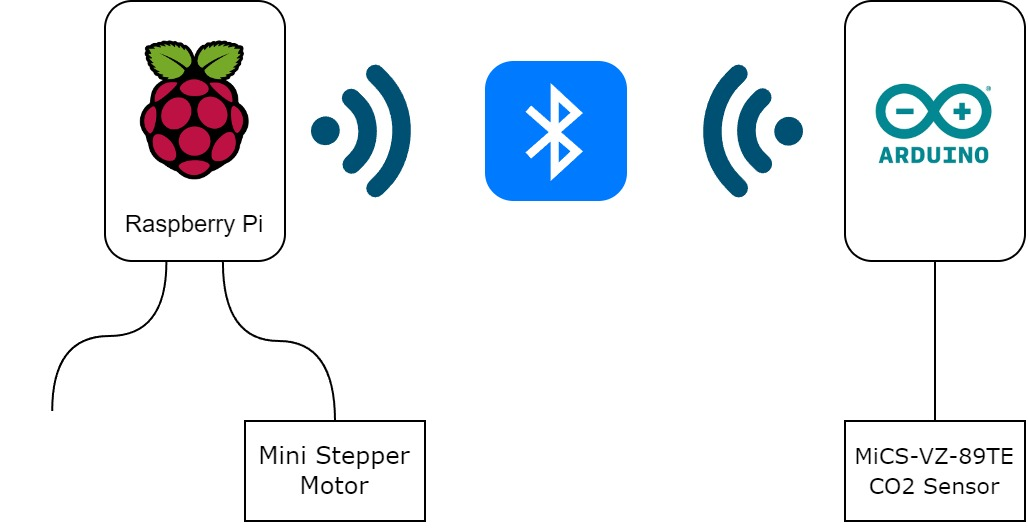
\includegraphics[height=70mm]{images/schema_technologien.jpg}
	\centering
	\caption{system description}
	\label{fig:system}
\end{figure}






